\documentclass{jsarticle}

%----------------------------------
% 文章の中に 画像を入れるための設定
%----------------------------------
\usepackage[dvipdfmx]{graphicx}

%----------------------------------
% 自分の作る文章の題
%----------------------------------
\title{上腕三頭筋の働きと鍛え方}

%---------------------------------- 
% 文書を作った日
%----------------------------------
\date{\today}

%----------------------------------
% 自分の名前を入れる
%----------------------------------
\author{山 根 千 佳}

%---------------------------------------------------
% 文書のスタイルを決める設定
%---------------------------------------------------
\usepackage[height=26cm,width=16cm]{geometry}

%-----------------------------------
% 以上で下準備は終わりです.
% ここから表示される文章を作成していきます.
%-----------------------------------
\begin{document}

%----------------------------------------
% 文章に上に、上記で記述したタイトル、
% 文書を作成した日にち, 著者の名前を書き込みます.
%
% (注)\maketitle をはずせば, タイトル, 日にち,著者名は文書に挿入されません.
%----------------------------------------

\maketitle

%--------------------------------------------
% 主な内容はここから
%--------------------------------------------

\section{目的}
本レポートは、上腕二頭筋と上腕三頭筋の収縮が、腕の曲げ伸ばし運動にどのように作用しているのかを解明することを目的とした。具体的には、腕の曲げ伸ばし運動が遅い場合と速い場合の2パターンにおいて、筋電位の変化と腕の各関節の位置変化を同時に計測した。これにより、上腕二頭筋と上腕三頭筋の筋電位の変化と腕の曲げ伸ばしのタイミングを比較し、それぞれの筋収縮と腕の伸縮にどのような相関があるか調べた。

\section{実験方法}
被験者は、膝をついた状態で座り、腕を床と水平に繰り返し曲げ伸ばしした。
計測は、腕の伸縮をゆっくり行った場合と、早く行った場合との2パターンについて行った。
本実験における被験者は1人であった。
                                                                                                                                                                                                                                                                                                                                                                                                                                                                                                                                                                                                                                                                                                                                                                                                                                                                                                                                                                                                                                                                                                                                                                                                                                                                                                                                                                                                                                                                                                                                                                                                                                                                                                                                                                                                                                                                                                                                                                                                                                                                                                                                                   
\subsection{計測実験}
実験には、MotionCapture(ライブラリ社 MoveTR)と筋電計(ロジカルプロダクト社)を用いた。
MotionCaptureでは、被験者の運動の様子を真上からカメラで撮影し、肩、肘、手首の3点に貼付した反射マーカーの位置を200 fpsで計測した。
筋電計は上腕二頭筋および上腕三頭筋に貼付し、サンプリング周波数1000 Hzで各筋電位データを取得した。

\subsection{取得データの解析}
筋電データには、1〜40 Hzのバンドパスフィルタ(三次バターワース)をかけた。その後、フィルタを通すことで生じる位相のずれをなくすために、出力信号の時間を反転したものを、同じ特性のフィルタにかけ、再度時間を反転した。
時刻$t$における筋肉の活動度$a(t)$は、次式で評価した。
$$a(t) = \frac{1}{\Delta T} \int_{t-\frac{\Delta T}{2}}^{t+\frac{\Delta T}{2}} |E(t)|dt $$
として求めた。つまり、ある時刻$t$における筋肉の活動度を、その前後$\Delta T = 10$ [ms]の筋電位の平均値を$a(t)$とした。

\clearpage
\section{結果・考察}

\begin{figure}[htbp]
	\begin{center} %センタリングする
		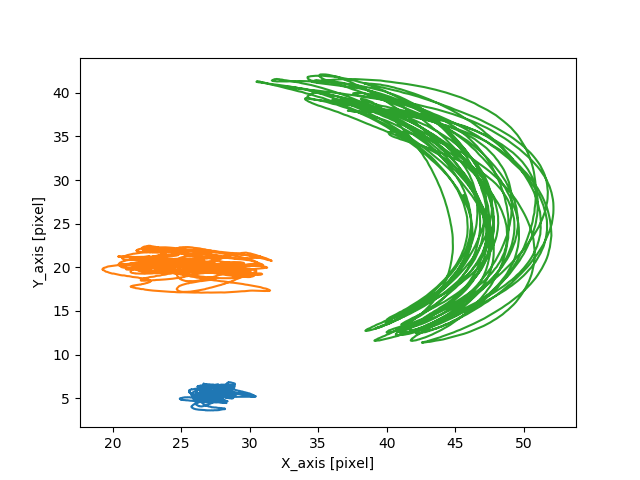
\includegraphics[width=12cm]{graph_image/slow_kidou.png}
		\caption{腕の3関節の軌道} %タイトルをつける
		\label{fig:kidou} %ラベルをつけ図の参照を可能にする
	\end{center}
\end{figure}

\begin{figure}[htbp]
(a)

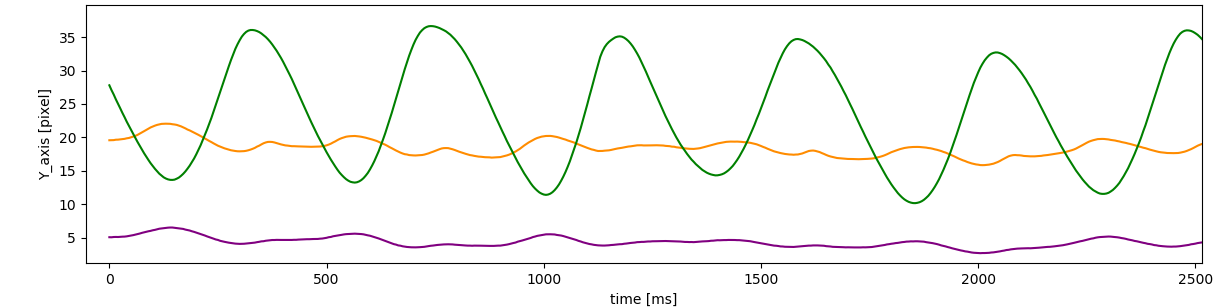
\includegraphics[width=17cm]{graph_image/fast_position.png}

(b)	

		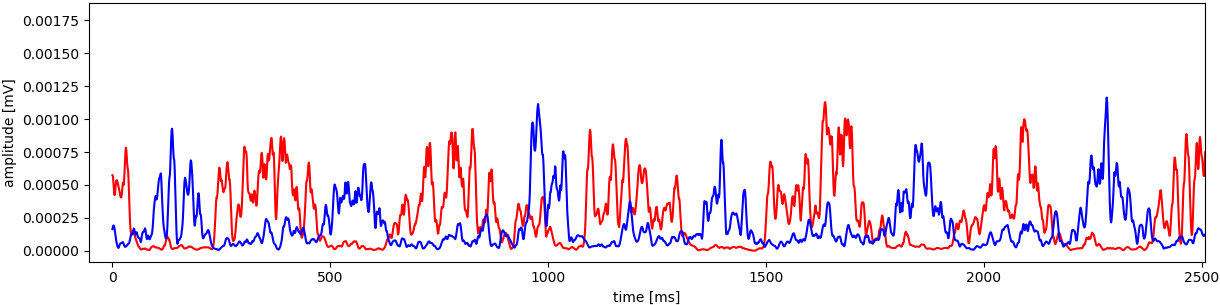
\includegraphics[width=17cm]{graph_image/fast_EMG.png}
		\caption{腕の曲げ伸ばし速度が遅い時の筋電データ。(a)は各関節の位置変化、(b)は筋電データである。}
		\label{fig:fast}	

\end{figure}
\clearpage

\begin{figure}[htbp]
	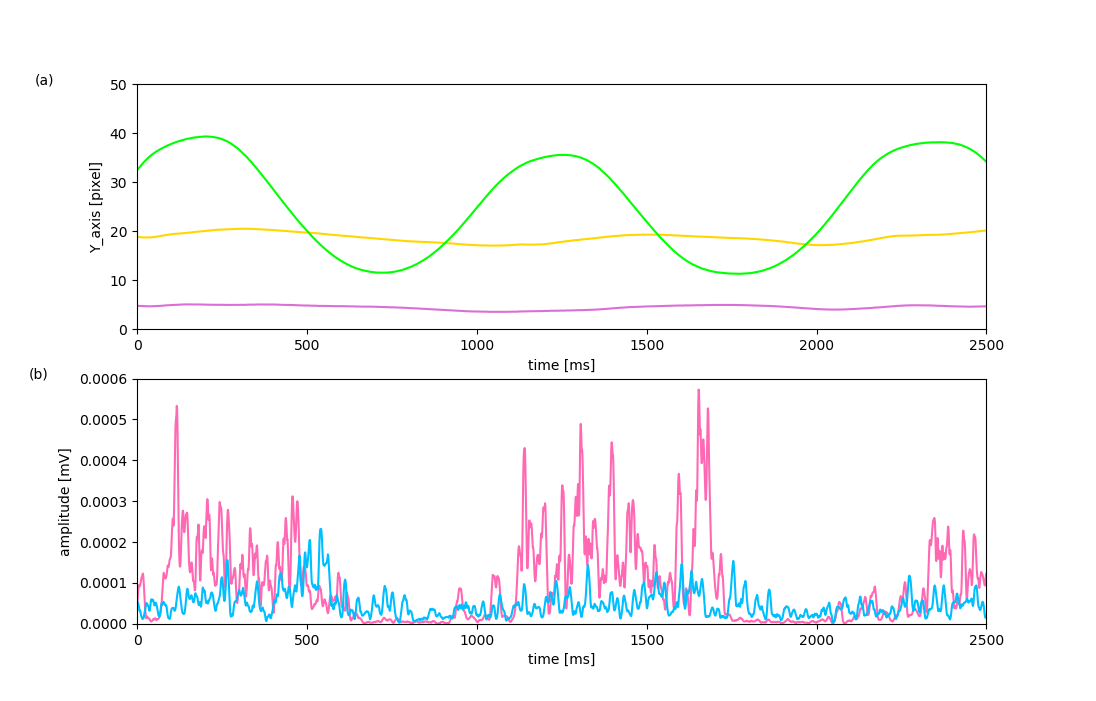
\includegraphics[width=17cm]{graph_image/slow_position_EMG.png}
	\caption{腕の曲げ伸ばし速度が遅い時の筋電データ。(a)は各関節の位置変化、(b)は筋電データである。}
	\label{fig:slow}		
\end{figure}

図\ref{fig:kidou}はゆっくりと腕の曲げ伸ばし運動を行った場合の、各関節の位置変化を示す。
水色、オレンジ、黄緑はそれぞれ、肩、肘、手首の軌道を示している。
図\ref{fig:fast}、\ref{fig:slow}は、それぞれ腕の曲げ伸ばしが速い場合と遅い場合での計測結果を示す。
各図の(a)、(b)はそれぞれ腕の各関節におけるY軸方向の位置変化、および上腕二頭筋と上腕三頭筋の筋電位を表し、(a)の紫、黄色、緑はそれぞれ肩、肘、手首の位置変化、(b)の赤、青はそれぞれ上腕二頭筋、上腕三頭筋の筋電位である。

図\ref{fig:fast}は、腕を速く曲げ伸ばしした場合の筋電位データである。上腕二頭筋の筋活動は、腕を伸ばしている途中から腕を曲げ終わる少し前までにかけて、大きくなるという規則性が見られた。つまり、腕を曲げる前に筋活動が発生することで上腕三頭筋が収縮し、上腕骨と橈骨が近づくことで、腕が伸びると推測できる。
一方、上腕三頭筋の筋活動は、腕を曲げきる少し前から、腕を伸ばしている途中までのタイミングで大きくなっていた。つまり、腕を伸ばす前に筋活動が発生することで上腕三頭筋が収縮し、上腕骨と尺骨が近づくことで、腕が伸びると推測できる。

図\ref{fig:slow}は、腕を遅く曲げ伸ばしした場合の筋電位データである。上腕二頭筋の筋活動は、腕を伸ばす途中から腕を曲げ終わる少し前までにかけて大きくなっており、速く曲げ伸ばしした場合と同様の規則性が見られた。このことからも、腕を曲げる前に筋活動が発生することで上腕二頭筋が収縮し、上腕骨と橈骨が近づくことで、腕が伸びると推測できる。
一方、上腕三頭筋では、約100msと短時間ではあるが、腕を曲げる途中で筋活動が大きくなっていた。このことからも、腕を伸ばす前に筋活動が発生することで上腕三頭筋が収縮し、上腕骨と尺骨が近づくことで、腕が伸びると推測できる。
しかし、腕の伸縮が速いときほど筋電位の振幅の変化が見られなかった。

以下に、腕の曲げ伸ばしが速い場合と遅い場合で、上腕三頭筋の筋活動の様子が異なる理由について考える。上腕三頭筋は上腕二頭筋の反対側に存在する筋肉である。このことから、上腕三頭筋は、上腕二頭筋により生じる腕を曲げる力と逆方向の力を発生させることで、腕の曲げ速度を抑えるブレーキの役割があると推測される。上腕三頭筋の筋活動を腕の伸縮が速いときと遅い時とで見比べると、遅い時には腕を曲げる途中で大きな筋活動が100msほど発生して、それ以降すぐに小さくなっていた。一方、速い時では、腕を曲げきる少し前から伸ばしている途中まで大きな筋活動がを維持していた。このことから、腕を伸ばすための筋電位の後に、続けてブレーキをかけるための筋活動が発生すると考えられる。また、この役割が発揮されるのは腕の曲げ伸ばし速い場合だけであり、遅い場合には、この機能がほぼ必要ないため、筋活動があまり時間変化しなかったと考えらる。 

これらの結果から、腕を曲げ伸ばしには、それぞれ上腕二頭筋の収縮、上腕三頭筋の収縮が必要である。また、上腕三頭筋は、腕を伸ばす役割の他に、腕が曲がる速度を抑えるブレーキの役割も担っていると考えられる。


\begin{thebibliography}{9}
	\bibitem{reference1} 「3D 踊る肉単」 河合良訓,原島広至 pp.xiv, 38
\end{thebibliography}
%--------------------------------------------
% 文章これまで.
%--------------------------------------------
\end{document}
